\section{The Wavelet Tree}
The Wavelet Tree is a tree structure of bitmaps.
It was invented by Grossi, Grupta and Vitter~\citeA{Grossi:2003:HET:644108.644250} in 2003.
In its basic form, it is a balanced binary tree of bitmaps, encoding a \textit{sequence} or \textit{string} $S[1,n] = c_1c_2c_3 \ldots c_n$ of \textit{symbols} or \textit{characters} $c_i \in \Sigma$, where $\Sigma = [1 \ldots \sigma]$ is the \textit{alphabet} of $S$, in such a way that it supports a number of fast queries on $S$.
A balanced wavelet tree over a string $S$ with alphabet $\Sigma$ will have height $h = \lceil \log \sigma \rceil$, and $2 \sigma - 1$ nodes, with $\sigma$ of those as leaf nodes and $\sigma - 1$ as internal nodes.
In this thesis, we use $\log$ as having base 2 unless otherwise noted.

With extensions, a wavelet tree can be used for efficient compression of $S$ while still supporting the same queries, although not as fast.
It has applications in many areas, from string processing to geometry, and can be used to represent, among others, a sequence of elements, a reordering of elements or a grid of points. 
When~\citeA{Grossi:2003:HET:644108.644250} invented the Wavelet Tree, it was a milestone in compressed full-text indexing even though it is mentioned little in the paper.
The wavelet tree has even been shown to be able to get close to a lower bound of compression called $k$th-order entropy encoding (see Section~\ref{sec:entropy}).

\subsection{Constructing the Wavelet Tree}
\label{sec:nodeconstruction}
The wavelet tree is constructed recursively, starting at the root node and going down, with each node in the tree receiving a string from its parent, except the root node that receives the full input string.
Let $S_{\mathit{parent}}$ of length $n_{\mathit{parent}}$ be the string passed to the node from the parent node or, in the case of the root node, the input string to the wavelet tree itself.
$\Sigma_{\mathit{parent}}$ is the alphabet over which $S_{\mathit{parent}}$ is defined where each entry in the alphabet, a \textit{character} or \textit{symbol}, has a position in the alphabet.
$\sigma_{\mathit{parent}}$ is the size of $\Sigma_{\mathit{parent}}$.
Each node stores a bitmap of size $n_{\mathit{parent}}$ as well as pointers to its left and right child nodes.

Each node calculates the middle character of $\Sigma_{\mathit{parent}}$ and uses that to set the bits in the bitmap and split $S_{\mathit{parent}}$ in two substrings $S_{\mathit{left}}$ and $S_{\mathit{right}}$, passing those on to the left and right child nodes.

Let $i = \left\lfloor\frac{\sigma}{2}\right\rfloor$ be the index of the middle of the alphabet $\Sigma_{\mathit{parent}}$.
$S_{\mathit{left}}$ is then the subsequence of $S_{\mathit{parent}}$ formed by the characters $c \in S_{\mathit{parent}}$ where $c \in \Sigma_{\mathit{parent}}[1 \ldots i] = \Sigma_{\mathit{left}}$.
$S_{\mathit{right}}$ is the subsequence of $S_{\mathit{parent}}$ formed by the characters $c \in S_{\mathit{parent}}$ where $c \in \Sigma_{\mathit{parent}}[i+1 \ldots \sigma_{\mathit{parent}}] = \Sigma_{\mathit{right}}$.
Alternatively, $S_{\mathit{left}}$ can be considered to be the subsequence of $S_{\mathit{parent}}$ where all characters $c \in \Sigma_{\mathit{right}}$ have been stripped out. Similarly $S_{\mathit{right}}$ can be considered the subsequence of $S_{\mathit{parent}}$ where all characters $c \in \Sigma_{\mathit{left}}$ have been stripped out.
This also means that the alphabets for the substrings $S_{\mathit{left}}$ and $S_{\mathit{right}}$ do not overlap, that is $\forall c \in \Sigma_{\mathit{left}}: c \notin \Sigma_{\mathit{right}}$ and vice versa.
The characters in the subsequences $S_{\mathit{left}}$ and $S_{\mathit{right}}$ occur in the same order they do in $S_{\mathit{parent}}$.
All these strings are not stored anywhere in the wavelet tree.
They are only used for the construction of the tree, but can later be reconstructed from the information stored in the bitmaps if need be.

Each bit in the bitmap corresponds to a character in the string $S_{\mathit{parent}}$.
If a character $c$ at position $p$ in $S_{\mathit{parent}}$ is in the left side of the alphabet $\Sigma_{\mathit{parent}}$, that is $c \in \Sigma_{\mathit{left}}$, the bit in the bitmap at position $p$ will be set to 0.
If instead $c \in \Sigma_{\mathit{right}}$, the bit at position $p$ will be set to 1.
Assuming the alphabet is in sorted order with regards to the \textit{greater than} ($>$) comparison operator, this can be computed as $c \in \Sigma_{\mathit{right}} = c > \Sigma[\lfloor\frac{\sigma}{2}\rfloor]$.
If the alphabet is not in sorted order, either lookups into the alphabet list or a mapping to and from an alphabet in sorted order will be needed to calculate whether a given character is on the left or right side of the alphabet.
The leaf nodes of a wavelet tree will appear in the same order as the characters they represent appear in the alphabet used.

This process continues recursively in each child node except where only one character is left in the alphabet of the input string of a node, $\sigma_{\mathit{parent}} = 1$.
That node is then considered a leaf node and needs not store a bitmap.
Each node in a wavelet tree can be considered a full wavelet tree for the string $S_{\mathit{parent}}$ it was passed from its parent node.

At each level in the tree at most \textit{n} bits are stored in the bitmaps in total, making $n \cdot h$ an upper bound to the total number of bits that a wavelet tree stores in its bitmaps.

The Wavelet Tree can theoretically be constructed in $O(n \cdot h)$ time as the sum of the lengths of the strings being processed at any single layer of the tree is the length of the input string to the tree.

An example of a Wavelet Tree can be seen in Figure~\ref{fig:WaveletTreeExample}.


The pseudo-code for the Wavelet Tree node construction algorithm is shown in Algorithm~\ref{alg:ConstructNode}. 
It is recursively defined, calling itself to construct the left and right sub-tree from the root node and down. At each recursion the algorithm splits the given alphabet in two halves and traverses the given string putting each character into a left or right partition based on whether the character was in the left or right half of the alphabet.

\figureBegin
\Tree
%root
[.adsfadaadsfaads\\001100000110001 !\qsetw{5cm} 
	%left child
	[.adadaadaad\\0101001001 !\qsetw{5cm}
		%left -> left,right child 
		[.aaaaaa !\qsetw{5cm} ] [.dddd !\qsetw{5cm} ]] 
	%right child
	[.sfsfs\\10101 !\qsetw{5cm} 
		%right -> left,right child
		[.ff !\qsetw{5.3cm} ] [.sss !\qsetw{5.3cm} ]]] 
\caption{Wavelet Tree on string \textit{adsfadaadsfaads} with alphabet $\Sigma = [\mathit{adfs}]$. Note that only the bitmaps are actually stored in the tree. The characters are annotations for ease of understanding.}	
\label{fig:WaveletTreeExample}
\figureEnd

\begin{algorithm}
\caption{Construction of nodes in the Wavelet Tree}
\label{alg:ConstructNode}
\begin{algorithmic}
\Function {ConstructNode} {S, $\Sigma$}
\If{$|\Sigma|$ = 1 or $|S|$ = 0}
	\State \Return
\EndIf
\State ($\Sigma_{\mathit{left}}$, $\Sigma_{\mathit{right}}$) $\gets$ $\Sigma$
\State SplitChar $\gets$ $\Sigma_{\mathit{left}}[\sigma_{\mathit{left}}]$
\ForAll {$c$ in $S$}
	\If {$c > $ SplitChar}
		\State $S_{\mathit{right}}$.Append($c$)
		\State Bitmap.Append(1)
	\Else
		\State $S_{\mathit{left}}$.Append($c$)
		\State Bitmap.Append(0)
	\EndIf
\EndFor
\State RightNode $\gets$ \Call {ConstructNode} {$S_{\mathit{right}}$, $\Sigma_{\mathit{right}}$}
\State LeftNode $\gets$ \Call {ConstructNode} {$S_{\mathit{left}}$, $\Sigma_{\mathit{left}}$}
\EndFunction
\end{algorithmic}
\end{algorithm}


\subsection{Access Query}
An access($p$) query is the query for what character $c$ us at position $p$ in the string $S$ the wavelet tree is constructed for.
The query can be answered by a single downward traversal of the wavelet tree.
Starting at the root node, an access query will look up the bit $b$ at position $p$ in the bitmap of the root node.
If $b$ is 0, we know that $c \in \Sigma_{\mathit{left}}$ and the algorithm must therefore traverse into the left child node.
If $b$ is 1, it means that $c \in \Sigma_{\mathit{right}}$ and the algorithm should traverse into the right child node instead.
Before we can continue down into the child node, we must know what position in the left (or right) substring $S_{\mathit{left}}$ (or $S_{\mathit{right}}$) the character $c$ has been mapped to.

If $b$ is 0, the position of $c$ in $S_{\mathit{left}}$ is the number of occurrences of 0 in the bitmap up to position $p$.
If $b$ is 1, the position of $c$ in $S_{\mathit{right}}$ is the number of occurrences of 1 in the bitmap up to position $p$.
This is also called rank$_0(p)$ or rank$_1(p)$ or the \textit{binary rank} of 0 or 1 in the bitmap up to position $p$.
In the most basic way it can be calculated using a linear scan of the bitmap making it $O(n)$, and since it is calculated one per level of the tree, the access query becomes $O(n \cdot h) = O(n \lceil \log \sigma \rceil)$.

Later in this thesis we will work on improving the running time of the binary rank query.
The result of the binary rank is then used as the position $p$ in the child node we traverse into.

We continue this traversal until we reach a leaf node that will then correspond to the character at the original position $p$ given to the query, where we can then return the character.

We have chosen not to implement or test access queries on our implementations of a wavelet tree.
We have done this to reduce the amount of code and testing needed and because the behaviour of rank (see Section~\ref{sec:rankDescription}) and access queries are so similar, e.g. both using binary rank, we believe implementing and testing only the more complicated rank query of these two will be representative enough of a real-world use case.

\subsection{Rank Query}
\label{sec:rankDescription}
The rank of a character $c$ in a string $S$ up to position $p$ is written as rank$_{p}(c)$ and is defined as the number of occurrences $o$ of $c$ in the substring $S[0, \ldots, p]$.

The rank query on a wavelet tree starts from the root of the wavelet tree and moves down through the tree until it hits the leaf node corresponding to the input character, much like the access query.
Also like the access query, each node calculates the binary rank of a character in the bitmap of the node and it is used as the positional parameter in the child node.
Unlike the access query, the rank query is looking at a specified character $c$ up to a position $p$, and whether it is the left or the right child node that is traversed into is decided by what $c$ is represented as in the bitmap of the current node and is calculated like it is when constructing the tree.

When the leaf node is reached, the binary rank calculated in the parent node is the rank of the input symbol up to the original input position.
Intuitively this makes sense because leaf nodes correspond to only one character and the rank of a character up to a position in a string containing only that character is the same as the position.
Figure~\ref{fig:RankDrawing} shows an example of how this concept works.
In the example, the rank query looks for the number of occurrences \textit{o} of the character $c = $ \textit{'a'} up to position $p = 10$.
It begins at the root and queries recursively towards the leaf node corresponding to \textit{'a'}. 
In each recursive call $p$ is set to $o_{parent}$ because only the 0s (or 1s) are mapped to the child node and $o$ indicates how many of these correspond to characters occurring before the original position $p_{parent}$.
In all the bitmaps \textit{'a'} is represented as 0 and in the root there are 6 occurrences of 0 up to position 10. 
In the left child node the algorithm then counts the number of 0s (3, making $o=3$) up to position 6 ($p=6$), and in the leaf it counts the number of 0s until position 3 of which there are 3 ($o=3, p=3$). 
This means that there are 3 occurrences of \textit{'a'} in \textit{S} up to position 10.

We have written the rank query as pseudo-code in Algorithm~\ref{alg:rank} using an object-oriented approach.

\begin{figure}
\center 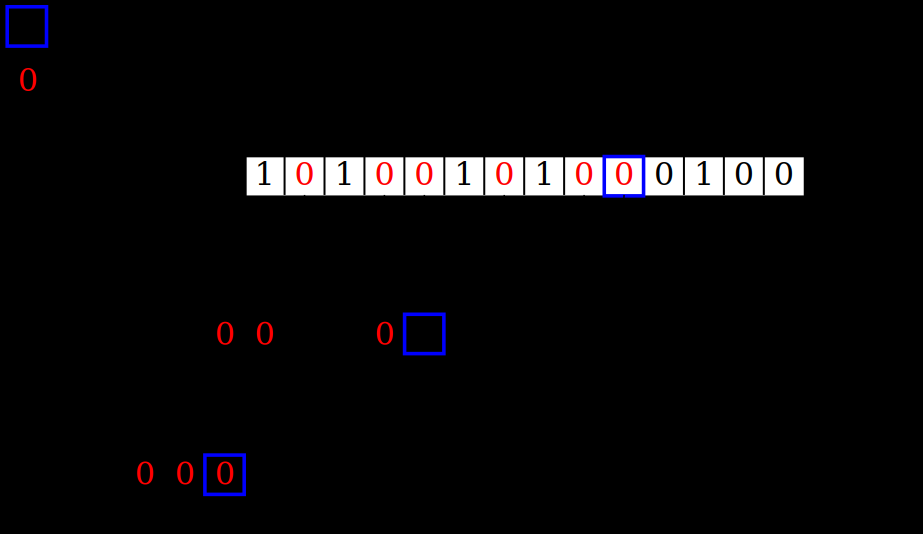
\includegraphics[width=1\textwidth]{RankDrawing}
\caption{Rank: This figure shows how the rank query algorithm works. 
In this example the algorithm looks for the number of occurrences \textit{o} of $c = $ \textit{'a'} until position $p = 10$.
It begins in the root and queries recursively towards the leaf node corresponding to \textit{'a'}.
The arrows indicate a mapping between the bitmaps.
In each recursion $p = o_{parent}$.
Each of the 0s before $p_{parent}$ in the parent node maps to bits before $p$ the child node.
In the root there are 6 0s up to position 10. 
In the left node there are 3 0s up to position 6
and in the leaf there are 3 0s up to position 3. This means there are 3 \textit{a}s up to position 10 in S.}
\label{fig:RankDrawing}
\end{figure}

\begin{algorithm}
\caption{Rank of character $c$ until position $p$}
\label{alg:rank}
\begin{algorithmic} 
\Function {Rank} {$c, p$}
\If{Self.IsLeaf}
\State \Return $p$
\EndIf
\State CharBit $\gets$ bit representing $c$ in bitmap of current node
\State o $\gets$ \Call {BinaryRank} {CharBit, $p$}
\If{CharBit $= 1$}
	\State Rank $\gets$ RightChildNode.\Call {Rank} {$c$, o}
\Else
	\State Rank $\gets$ LeftChildNode.\Call {Rank} {$c$, o}
\EndIf
\State \Return Rank
\EndFunction
\end{algorithmic}
\end{algorithm}


\subsection{Select query}
\label{sec:selectDescription}
The position of the $o$th occurrence of a character $c$ can be found with a select$_c(o)$ query.


The $i$th occurrence can be found with a traversal up through the wavelet tree starting at the leaf node corresponding to the character $c$ and ending at the root node.
This means it is necessary to find the leaf node corresponding to $c$.

The leaf node corresponding to a character $c$ can be found by a downward traversal of the tree, from the root to the leaf node without accessing any of the bitmaps.
Which child node, left or right, should be traversed is determined by computing whether $c \in \Sigma_{\mathit{left}}$ or $c \in \Sigma_{\mathit{right}}$.
If $c \in \Sigma_{\mathit{left}}$, the traversal continues in the left child node, otherwise it continues in the right child node.
The traversal continues until a leaf node is reached as that will be the leaf node corresponding to $c$.



After having found the leaf node the algorithm turns to do the upward traversal to find the position of the $i$th occurrence of $c$ in the bitmap of the root node.
This is done by finding the $o$th occurrence of 1 or 0, the bit representing $c$, in the bitmaps from the found leaf node to the root node, the $o$th occurrence of 1 or 0 being the bitmap entry corresponding to the $i$th occurrence of $c$ in $S$.
$o$ for a node $v$ is the position of the bit representing $c$ in the bitmap of the child node of $v$ that contains $c$.
$o$ is calculated for each node during the upward traversal and increases (or at least does not decrease) as each bitmap higher up the tree corresponds to more and more of the original input string.
To know which bit, 1 or 0, to look for the $o$th occurrence of, the algorithm must know which bit $c$ has been mapped to in those bitmaps.
Starting at the leaf node corresponding to $c$, it can be computed which bit in the bitmap of the parent node represents all characters in this node, among them $c$, by comparing the left or right child node pointer of the parent node with the address of this node.
If the right child pointer of the parent node points to the current node, then the current node is the right child of its parent node and $c$ and the rest of the characters in this node will be represented by a 1 in the bitmap of the parent node, otherwise it will be represented by a 0.

Having found the bit representing $c$ in the parent node, the algorithm will look for the position of the $o$th occurrence of that bit in the bitmap of the parent.
This is also called select$_1(o)$ or select$_0(o)$ or the \textit{binary select} of 1 or 0 of the bitmap.
It can be implemented as a linear scan of the bitmap, but this is inefficient and later in this thesis we will look at how to improve the running time of binary select.
The position of this occurrence is then the new $o$ parameter for the next step up the tree.

In Algorithm~\ref{alg:select}, we display pseudocode for select queries.
\textproc{GetLeaf} is the function performing the initial downward traversal to find the leaf node corresponding to the character $c$.
\textproc{SelectRec} is the function performing the upward traversal, finding the (varying) $o$th occurrences of 1 or 0 in the bitmaps up the tree, in a recursive manner.
\textproc{Select} is the function computing the select$_{c}(o)$ query on the wavelet tree.
It initiates the downward traversal via \textproc{GetLeaf} and then the upward traversal via \textproc{SelectRec}.

An example of how the intuition behind why \textproc{Select} works is shown in Figure~\ref{fig:SelectDrawing}.
In the example the algorithm looks for the position of the 3rd occurrence of \textit{a}.
It looks of either 0 or 1 based on how a is represented in the bitmap of the current node. In this example \textit{a} is always represented as 0.
Select starts in the leaf of \textit{a} where $p = 3$ and $o = 3$ and moves recursively towards the root. In each recursive call $o_{parent} = p_{child}$, meaning that $p_{child}$ becomes the occurrence Select looks for in the parent. In this example Select therefore looks for the position of the 3rd occurrence of 0 in the parent of the leaf, which is 5. In the root it then looks for the position of the 5th occurrence of 0 which is 9 corresponding to the position of the 3rd \textit{a} in \textit{S}.

\begin{algorithm}
\caption{Select}
\label{alg:select}
\begin{algorithmic} 
\Function {Select} {$c$, Occurrence}
\State Leaf $\gets$ \Call{GetLeaf}{c}
\If{Leaf is a right child node}
	\State CharBit $\gets 1$
\Else
	\State CharBit $\gets 0$
\EndIf
\State \Return Leaf.Parent.\textproc{SelectRec}(CharBit, Occurrence)
\EndFunction

\vspace{5mm}

\Function {SelectRec} {CharBit, Occurrence}
\State Position $\gets$ \textproc{BinarySelect}(CharBit, Occurrence)
\If{Self is the root node}
	\State \Return Position
\EndIf
\If{Self is a right child node}
	\State CharBit $\gets 1$
\Else
	\State CharBit $\gets 0$
\EndIf
\State \Return Parent.\textproc{SelectRec}(CharBit, Position)
\EndFunction

\vspace{5mm}

\Function {GetLeaf} {$c$}
\If{Self.isLeaf}
	\State \Return Self
\EndIf
\If{$c \in \Sigma_{\mathit{right}}$}
	\State \Return RightChild.GetLeaf($c$)
\Else
	\State \Return LeftChild.GetLeaf($c$)
\EndIf
\EndFunction
\end{algorithmic}
\end{algorithm}

\begin{figure}
\center 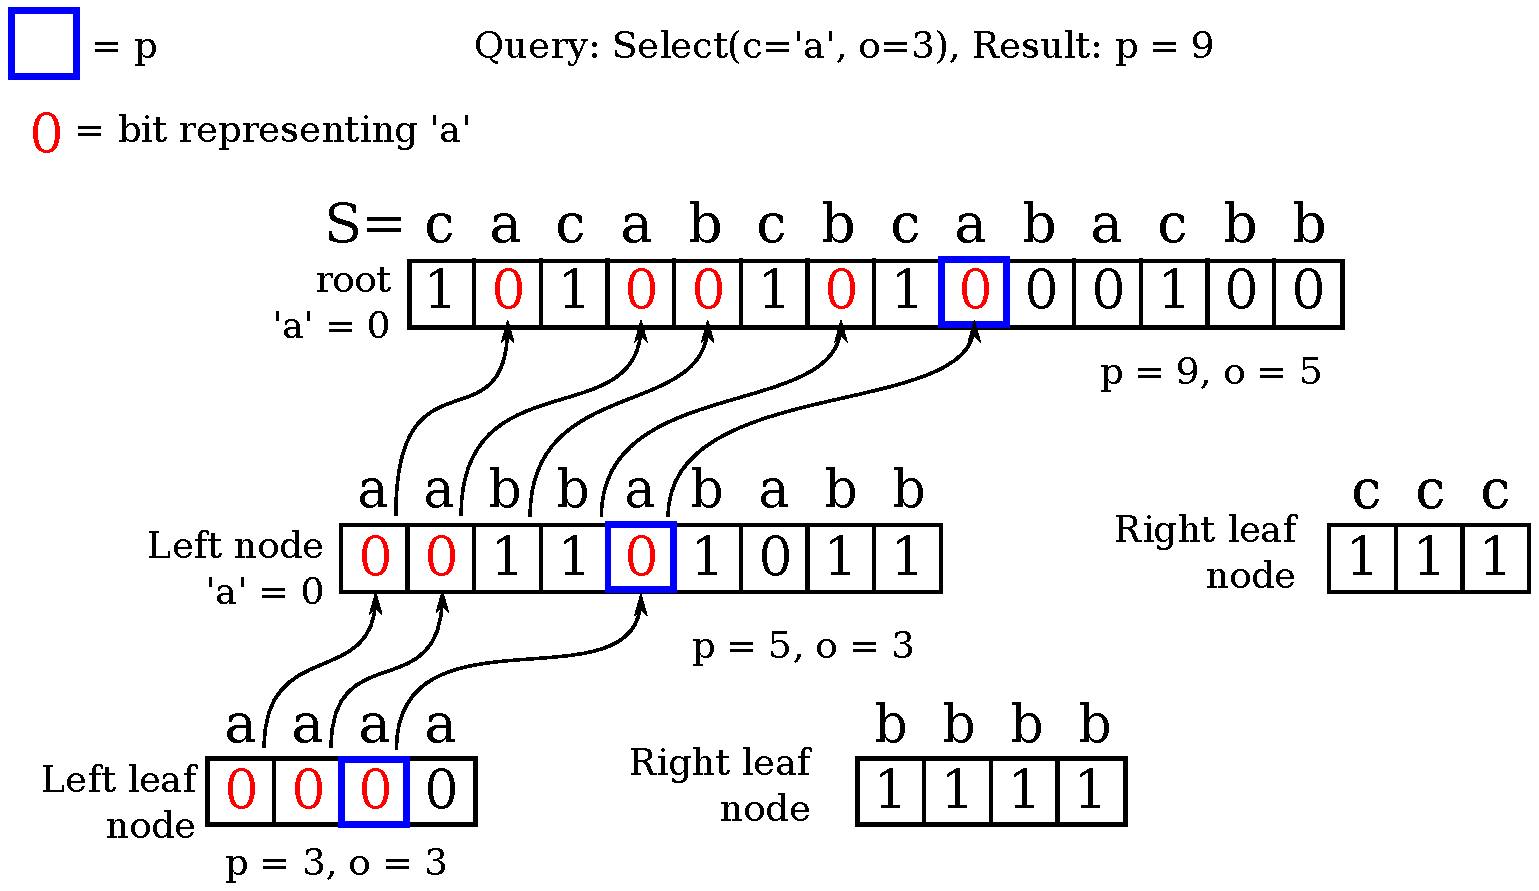
\includegraphics[width=1\textwidth]{SelectDrawing}
\caption{Select: This figure shows how the select algorithm works. 
In this example Select looks for the position of the 3rd occurrence of \textit{a} which is represented as 0 in the leaf.
Select starts in the leaf of \textit{a} where $p = 3$ and $o = 3$ and moves recursively towards the root. Along the way Select looks for the position of the 3rd occurrence of 0 in the parent of the leaf, which is 5, ($p=5, o=3$) and in the root it then looks for the position of the 5th occurrence of 0 which is 9, ($p=9, o=5$)  corresponding to the position of the 3rd \textit{a} in \textit{S}.}
\label{fig:SelectDrawing}
\end{figure}

